\documentclass{article}

\usepackage{polski}
\usepackage[utf8]{inputenc}
\usepackage{booktabs}
\usepackage{graphicx}
\usepackage{float}
\usepackage{geometry}
\usepackage{moreverb}
\geometry{
	a4paper,
	total={170mm,257mm},
	left=35mm,
	right=35mm,
	top=35mm,
	bottom = 25mm
}


\begin{document}
	\newgeometry{tmargin=2cm, bmargin=2cm, lmargin=2cm, rmargin=2cm}
	
	\begin{titlepage}
		\center
		\newcommand{\HRule}{\rule{\linewidth}{0.5mm}}
		
		\textsc{\LARGE Politechnika Wrocławska}\\[1.5cm]
		\textsc{\Large Projekt}\\[0.5cm] 
		\textsc{\large Architektura Komputerów 2}\\[0.5cm] 

		\HRule \\[0.4cm]
		{ \huge \bfseries System lokalizacji GPS z wykorzystaniem komputera Raspberry Pi 2}\\[0.4cm]
		\HRule \\[1.5cm]
		
		\begin{minipage}{0.4\textwidth}
			\begin{flushleft} \large
				\emph{Authors:}\\
				Rafał \textsc{Pieniążek} 
				\\ Jakub \textsc{Pomykała}
			\end{flushleft}
		\end{minipage}
		~
		\begin{minipage}{0.4\textwidth}
			\begin{flushright} \large
				\emph{Supervisor:} \\
				Dr inż. Jędrzej \textsc{Ułasiewicz} 
			\end{flushright}
		\end{minipage}\\[4cm]

		{\large \today}\\[3cm]
		
		\vfill
		
	\end{titlepage}

\newpage
	
\section{Wstęp}
	\subsection{Cel projektu}
	Zaprojektować system określania pozycji z wykorzystaniem modułu GPS i komputera Raspberry PI 2. System ma wyświetlać pozycję na wyświetlaczu LCD.
	\subsection {Etapy projektu}
	\begin{itemize}
	\item Zapoznanie się z komputerem Raspberry PI 2
	\item Zapoznanie się z układem lokalizacji satelitarnej GPS Global TOP FGPMMOSL3
	\item Zaprojektowanie połączenia komputera z  modułem lokalizacji, wyświetlaczem LCD.
	\item Opracowanie programu obsługi lokalizatora i wyświetlacza
	\item Testy
	\end{itemize}
	\subsection{struktura kodów \textit{NMEA}}
		NMEA jest protokołem komunikacji wykorzystywanym głownie w nawigacji morskiej. Dane przesyłane są w postaci sekwencji kodów oddzielonych przecinkami. Każde takie zdanie zawiera informacje m.in. o identyfikatorze wiadomości, czasie UTC, długości i szerokości geograficznej (wraz z identyfikatorami półkuli północnej/południowej oraz wschodniej/zachodniej),  ilości satelitów użytych do ustalenia położenia. Poniżej przedsationo przykładowy kod:
		\begin{verbatim}
		$GPGGA,123519,5107.038,N,01731.000,E,1,08,0.9,545.4,M,46.9,M,,*47
		\end{verbatim}
    \subsection{Odczyt danych z modułu GPS }
    
	   Po podłączeniu modułu lokalizacji do komputera Raspberry Pi poprzez złącze szeregowe możliwe jest odczytywanie danych w sposób analogiczny do czytania z pliku. W związku z tym użycie komendy bashowej:
	   	\begin{verbatim}
	   	"cat /dev/ttyAMA0"
	   	\end{verbatim} 
	   	pozwoliło na wypisanie danych przesyłanych przez GPS na ekran konsoli.
\section{Opis projektu}
	\subsection{Wykonanie połączeń układu}
		Pierwszym etapem prac było zapoznanie się z dokumentacją techniczną modułu lokalizacji. Po przeanalizowaniu odpowiednich wyprowadzeń rozpoczęto fizyczny montaż modułu do płytki prototypowej. Podczas wykonywania tych czynności napotkano techniczny problem wykonania połączeń lutowanych. Mały rozmiar wyprowadzeń oraz niestandardowy rozmiar uniemożliwił użycia jakiejkolwiek podstawki do zamocowania w płytce prototypowej. Konieczne było ręczne przylutowanie wyprowadzeń przy zastosowaniu precyzyjnej lutownicy. Sprzęt jakim dysponowano był nieodpowiedniej klasy i mocy, obawiano się przegrzania i uszkodzenia układu. Problem został rozwiązany dzięki wykorzystaniu sprzętu Politechniki Wrocławskiej. Podłączenie kolejnych elementów układu nie sprawiło większych problemów. Poniżej przedstawione zostały schematy połączeń, oraz wizualizacja układu.
		
			\begin{figure}[H]
				\centering
				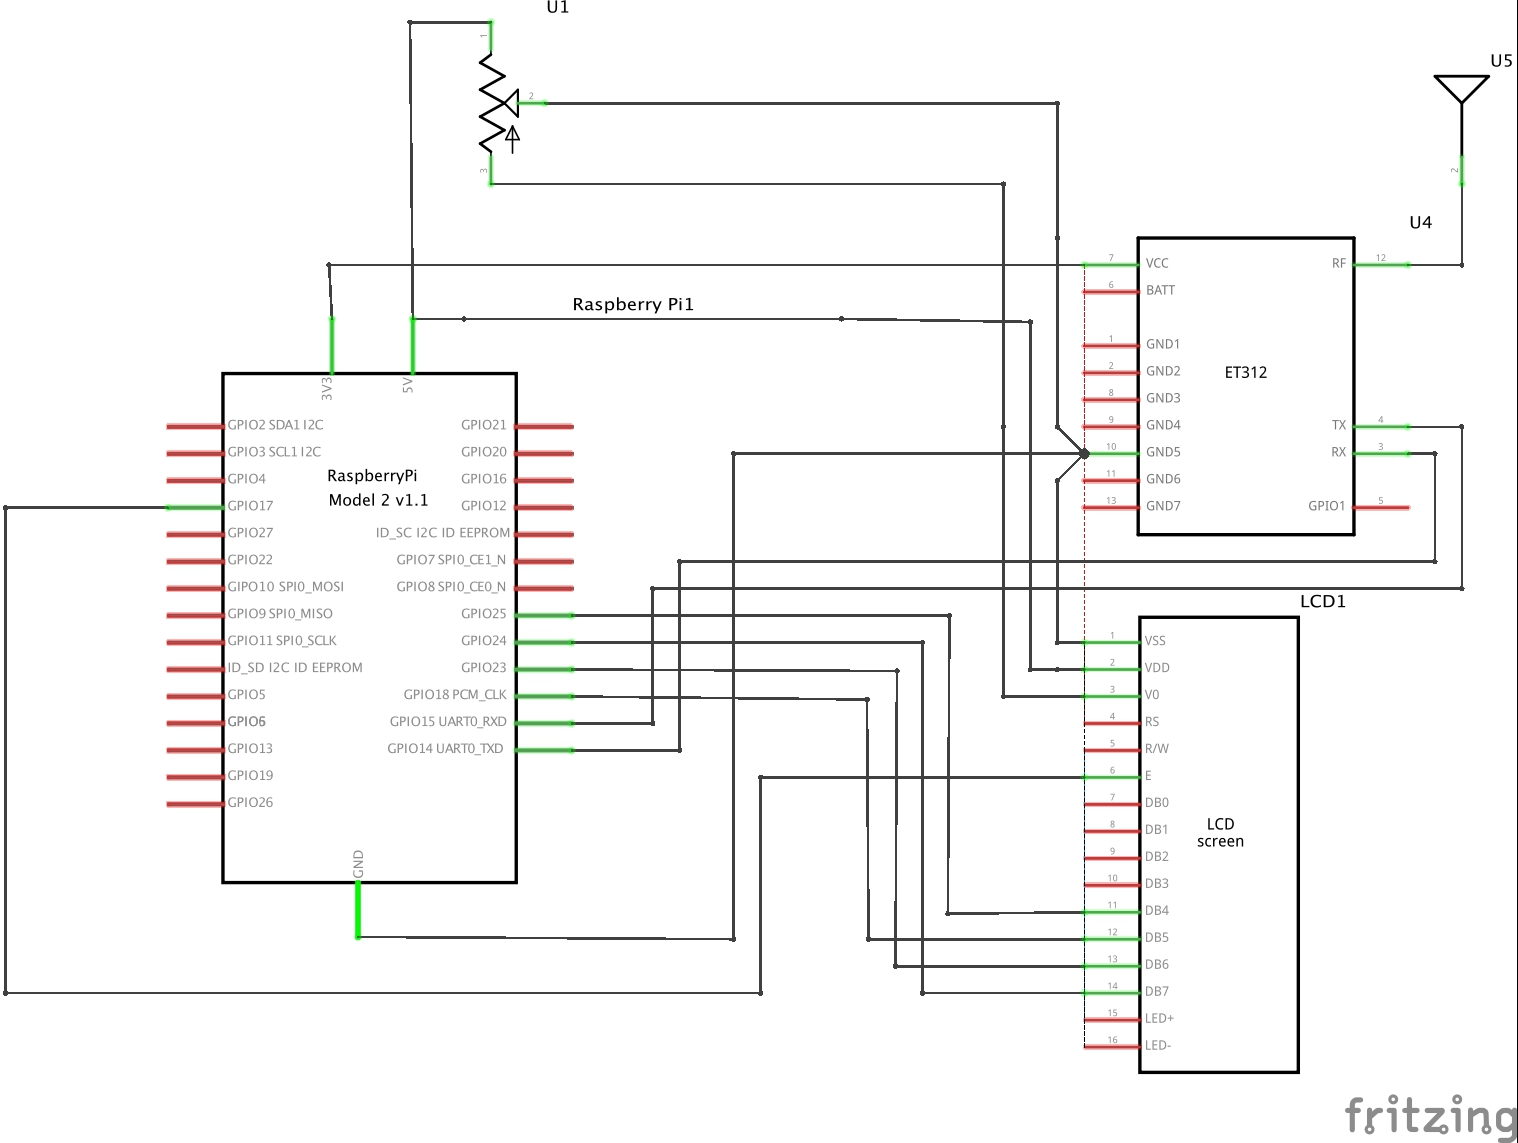
\includegraphics[width=0.9\linewidth]{schemat-podlaczenia_schem.jpg}
				\caption{Schemat podłączeń}
			\end{figure}
			
			
			\begin{figure}[H]
				\centering
				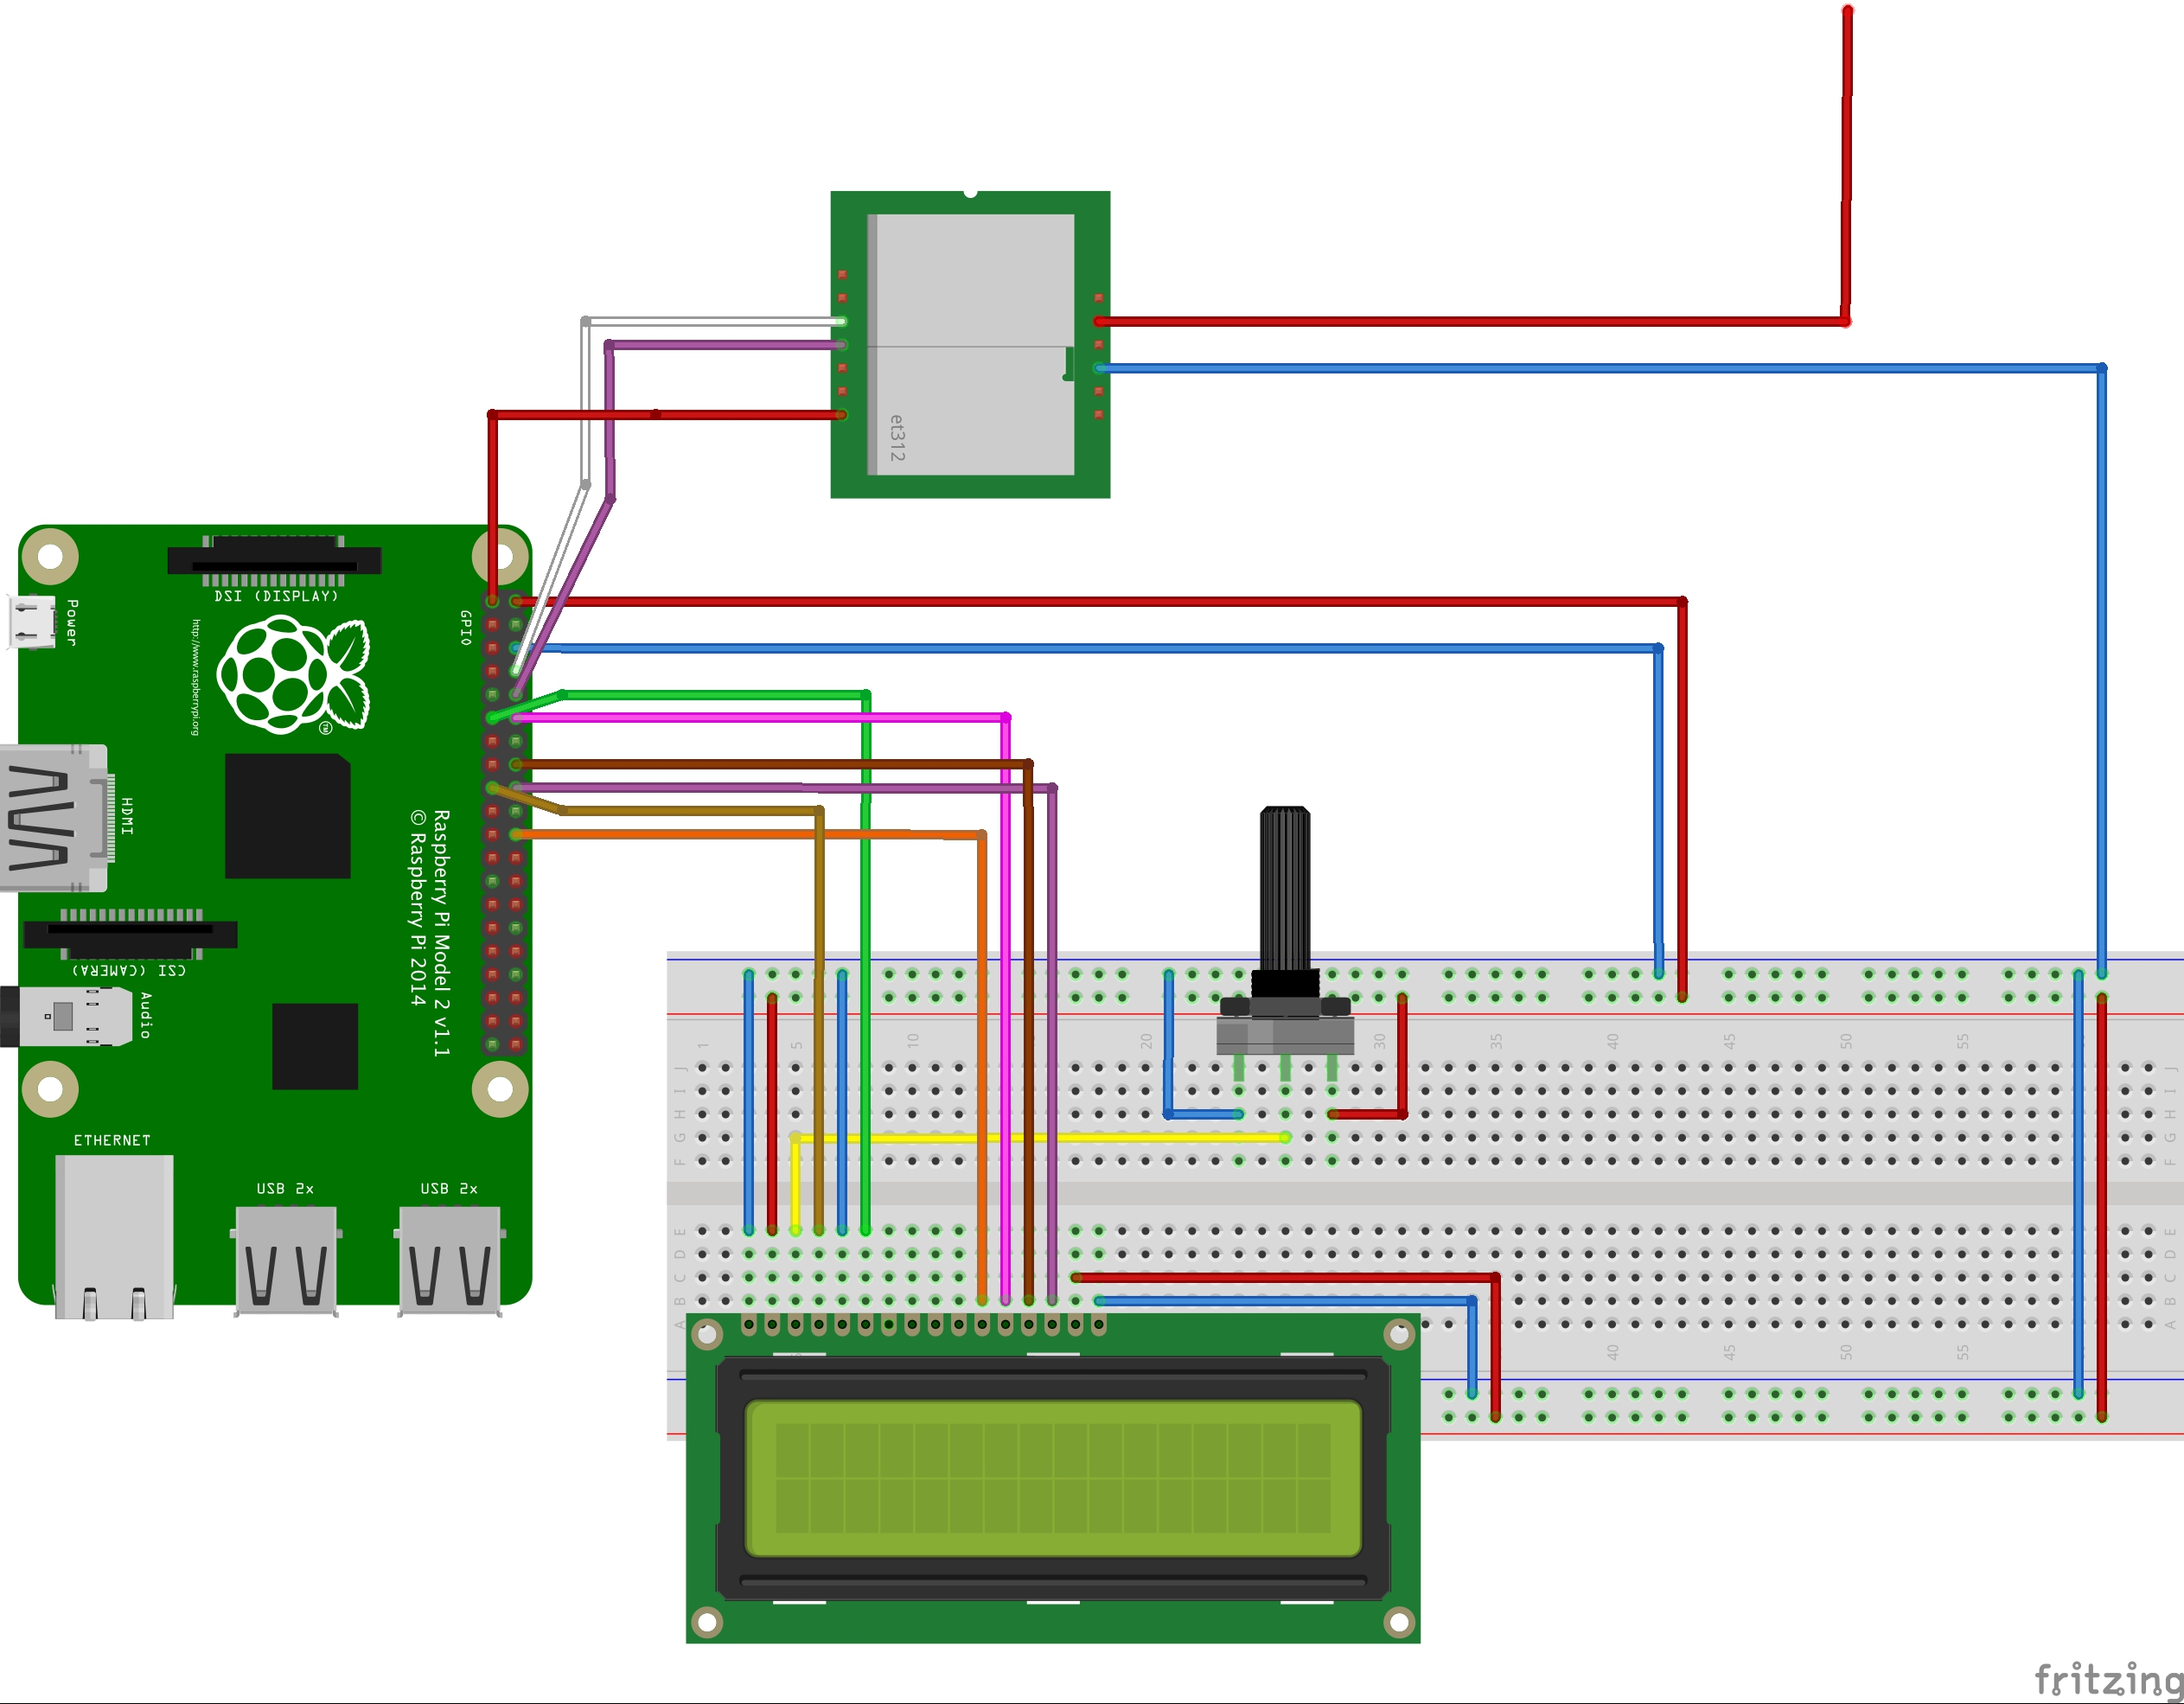
\includegraphics[width=0.9\linewidth]{schemat-podlaczenia_bb.jpg}
				\caption{Wizualizacja połączeń}
			\end{figure}
			
	\subsection{Implementacja programu}
		Do implementacji programu wykorzystano język C. W pierwszej kolejności oprogramowany został moduł wyświetlacza LCD. Wykorzystano bibliotekę udostępnioną dla komputerów Raspberry Pi - \textit{WiringPi}, a z niej moduł \textit{Lcd}. Poniżej przedstawiona została funkcja inicjalizująca wyświetlacz.
		%uwaga z wyrownaniem kodu zrodlowego, wplywa to na wyglad dokumentu po kompilacji
		\begin{verbatimtab}[4]
	int initLCD(){
		int lcd;
		if (lcd = lcdInit (2, 16,4, LCD_RS, LCD_E ,LCD_D4 , LCD_D5, LCD_D6,LCD_D7,0,0,0,0)){
			printf ("Nie udana inicjalizacja LCD! \n");
			return -1;
		}
		return lcd;
	}
		\end{verbatimtab}
		
		Na podstawie dokumentacji zaimplementowano  funkcję do ekstrakcji danych z kodów \textit{NMEA}. Funkcja ta parsuje ciągi znaków wczytane ze wejścia szeregowego, do którego podłączony jest moduł GPS. Następnie odczytane współrzędne wypisywanie są na LCD:
		\begin{verbatimtab}[4]
	void parseNmea(char Buffer[255])
	{
		if(Buffer[0] == '\$')
		{
		if (memcmp(Buffer+1,"GPGLL",5) == 0)
		{
			char *token = strtok(Buffer+6,",");
			char *lat;
			int i = 0;
			while(token != NULL)
			{
				switch(i)
				{
				case 0:
					printf(" Lat: %s ", token);
					lcdPosition(lcd,0,0); 
					lcdPuts(lcd, "Lat: ");
					lcdPuts(lcd, token);
				    break;
				case 2:
					printf(" Lng: %s ", token);
					lcdPosition(lcd,0,1); 
					lcdPuts(lcd, "Lng: "); 
					lcdPuts(lcd, token);
					break;		
			
				default:
					printf("----------- BLAD!\n");
					break;
				}
				i++;
				token = strtok(NULL,",");
				}
			printf("\n");
			}
		}
	}
	\end{verbatimtab}
	
	Kolejnym fragmentem przygotowanego programu jest funkcja odczytująca dane z wejścia szeregowego, do którego podłączony został układ lokalizacji. Wykorzystano funkcję \textit{serialOpen}  z biblioteki standardowej. Odczyt danych przekazywanych przez GPS bazuje na czytaniu z pliku. Konieczne jest podanie ścieżki, oraz prędkości odczytu. Następnie następuje zapętlenie programu; kolejno pobierany jest odpowiedni kod \textit{NMEA} i wywoływana wspomniana wcześniej metoda odpowiedzialna za parsowanie kodu i wyświetlanie danych na LCD.
	\begin{verbatimtab}[4]
	void startTracking()
	{
		char gps[65];
		int fd,flag=0; //uchwyt dla UART
		char arr[]="\$GPGGA";
		
		if((fd = serialOpen("/dev/ttyAMA0",9600)) < 0)
		{
			printf("%s\n", "Nie udalo sie podlaczyc do UART");
			return;
		} 
		else
		{
			printf("Podlaczono UART\n");
		}
		int i = 0;
		char buffer[255];
		while(1)
		{
		int c;
			if(c=serialGetchar(fd))
			{
				if(c != '\n')
				{
					buffer[i] = c;
				}
				else 
				{
					buffer[i] = '\0';
					parseNmea(buffer);
					i = -1;
				}
				i++;
			}
		}
	}
	\end{verbatimtab}
	
	Cały projekty kompilowano poniższym poleceniem:
	\begin{verbatim}
	gcc lcd.c -o lcd -lwiringPi -lwiringPiDev
	\end{verbatim}
	\subsection{Testowanie}	
	Początkowo testowano samo połączenie GPS z platformą Raspberry. Wykonanie komendy bashowej:
	\textit{"cat /dev/ttyAMA0"}
	pozwala na wypisanie nieprzetworzonych danych na ekran konsoli. Niestety pierwsze próby zakończyły się fiaskiem. Powodem był brak anteny. Okazało się, że moduł lokalizacji wykorzystany w projekcie nie jest w nią zaopatrzony. Konieczne było dolutownaie przewodu o odpowiedniej długości, do odpowiedniego wyjścia modułu. Po tych czynnościach udało się otrzymać dane o położeniu.
	Program został skompilowany i uruchomiony na platformie Raspberry. Po włączeniu modułu konieczne jest odczekanie pewnej ilości czasu na ustablizowanie połączenia. Czas ten nie jest dłuższy niż 5 minut. Po tym czasie dane o lokalizacji pojawiają się na LCD:
	
		\begin{figure}[H]
		\centering
		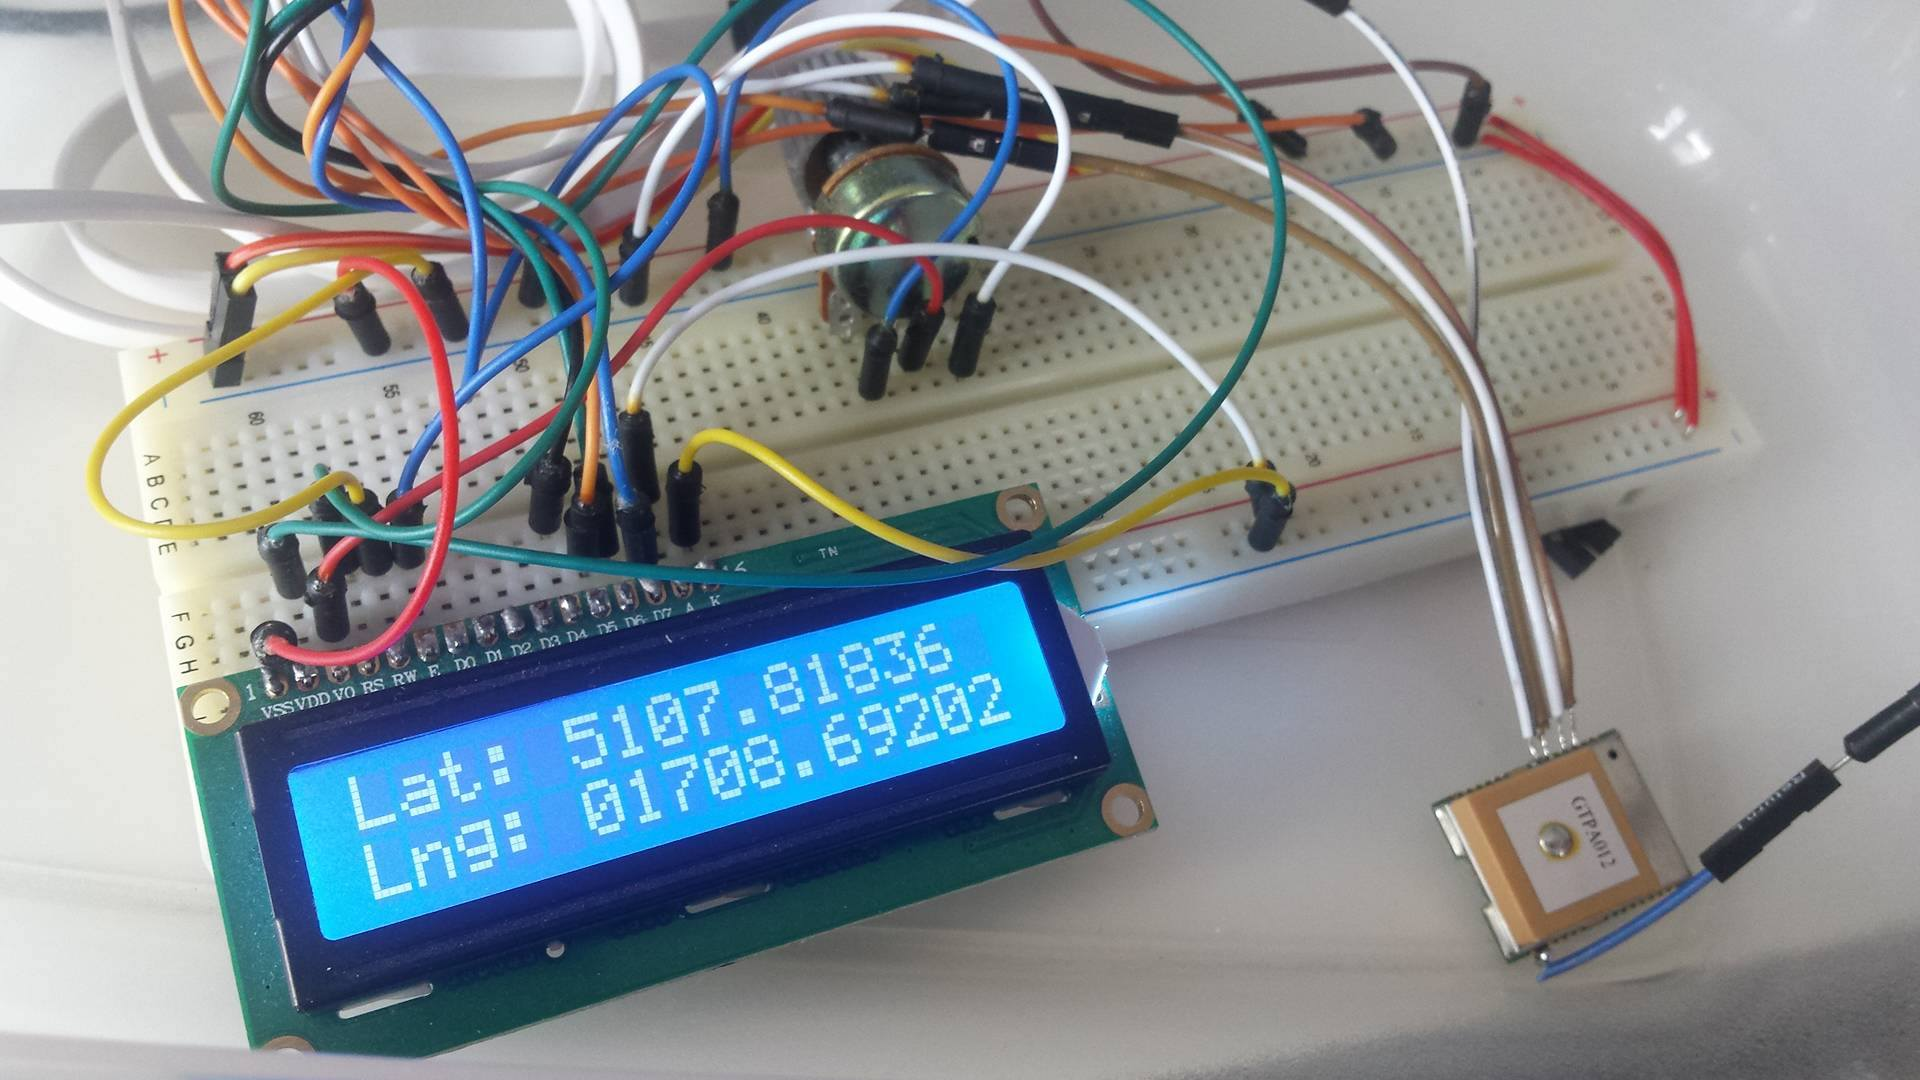
\includegraphics[width=0.9\linewidth]{efekt1.jpg}
		\caption{Uzyskany efekt}
		\end{figure}
\section{Podsumowanie}
	Realizacja projektu pozwoliła na zapoznanie się z formatem kodów \textit{NMEA}. Mnogość zagadnień teoretycznych obejmujących odczyt danych z portu szeregowego, wydobywanie danych z \textit{NMEA} obsługę LCD jak również cześć praktyczna dotycząca lutowania i fizycznych połączeń była ciekawym i interesującym doświadczeniem. Najbardziej pouczające było szukanie przyczyn braku danych o lokalizacji, pomimo poprawnego podłączania modułu. W pierwszym momencie sądzono, że moduł został uszkodzony z powodu zbyt dużej temperatury podczas lutowania wyprowadzeń. Dołączenie anteny rozwiązało ten problem.

\end{document}\documentclass{article}
